\documentclass[12pt,letterpaper]{article}
%\usepackage{preamble}

%\ProvidesPackage{preamble}

\usepackage{fullpage}
\usepackage[top=2cm, bottom=4.5cm, left=2.5cm, right=2.5cm]{geometry}
\usepackage{amsmath,amsthm,amsfonts,amssymb,amscd}
\usepackage{lastpage}
\usepackage{enumerate}
\usepackage{fancyhdr}
\usepackage{mathrsfs}
\usepackage{xcolor}
\usepackage{graphicx}
\usepackage{listings}
\usepackage{hyperref}
\usepackage{enumitem}
\usepackage{float}
\usepackage{fancyvrb}
\usepackage{color,soul}
\sethlcolor{lightgray}
 \usepackage{subfigure}
 \usepackage{textcomp}
\usepackage{siunitx}

\usepackage{graphicx}
\usepackage{array}

\usepackage[T1]{fontenc}
\usepackage[numbered,framed]{matlab-prettifier}
\hypersetup{%
  colorlinks=true,
  linkcolor=blue,
  linkbordercolor={0 0 1}
}

\let\ph\mlplaceholder % shorter macro
\lstMakeShortInline"

\lstset{
  style              = Matlab-editor,
  basicstyle         = \mlttfamily \small,
  escapechar         = ",
  mlshowsectionrules = true,
  xleftmargin=.01\textwidth, xrightmargin=.01\textwidth
}

\graphicspath{{./problem1_images}}

\pagestyle{fancyplain}
\headheight 35pt
\lhead{\userID}
\chead{\textbf{\Large Project \hwnumber}}
\rhead{\course \\ \today}
\lfoot{}
\cfoot{}
\rfoot{\small\thepage}
\headsep 1.5em




%%%%%%%%%%%%%%%%%%%%%%%%%%%%%%%%%%%%%%%%%%
%%%% Edit These for yourself
%%%%%%%%%%%%%%%%%%%%%%%%%%%%%%%%%%%%%%%%%%
\newcommand\course{Econ 672}
\newcommand\hwnumber{7}
\newcommand\userID{Ziming Huang}
\newenvironment{alphaparts}[0]{%
  \begin{enumerate}[label=\textbf{\Alph*}]
}{\end{enumerate}}


\begin{document}


\section*{Exercise}
\begin{enumerate}[label=\textbf{(\Alph*)}]  	
  	
%----A-----
\item 
The coarse sample function is as follow:
\textbf{AR Model} 
\lstinputlisting{functions/log_return_new.m}
%---B
\item Here is the graph of annualized RV with different sample frequency.
\begin{figure}[H]
	\centering
    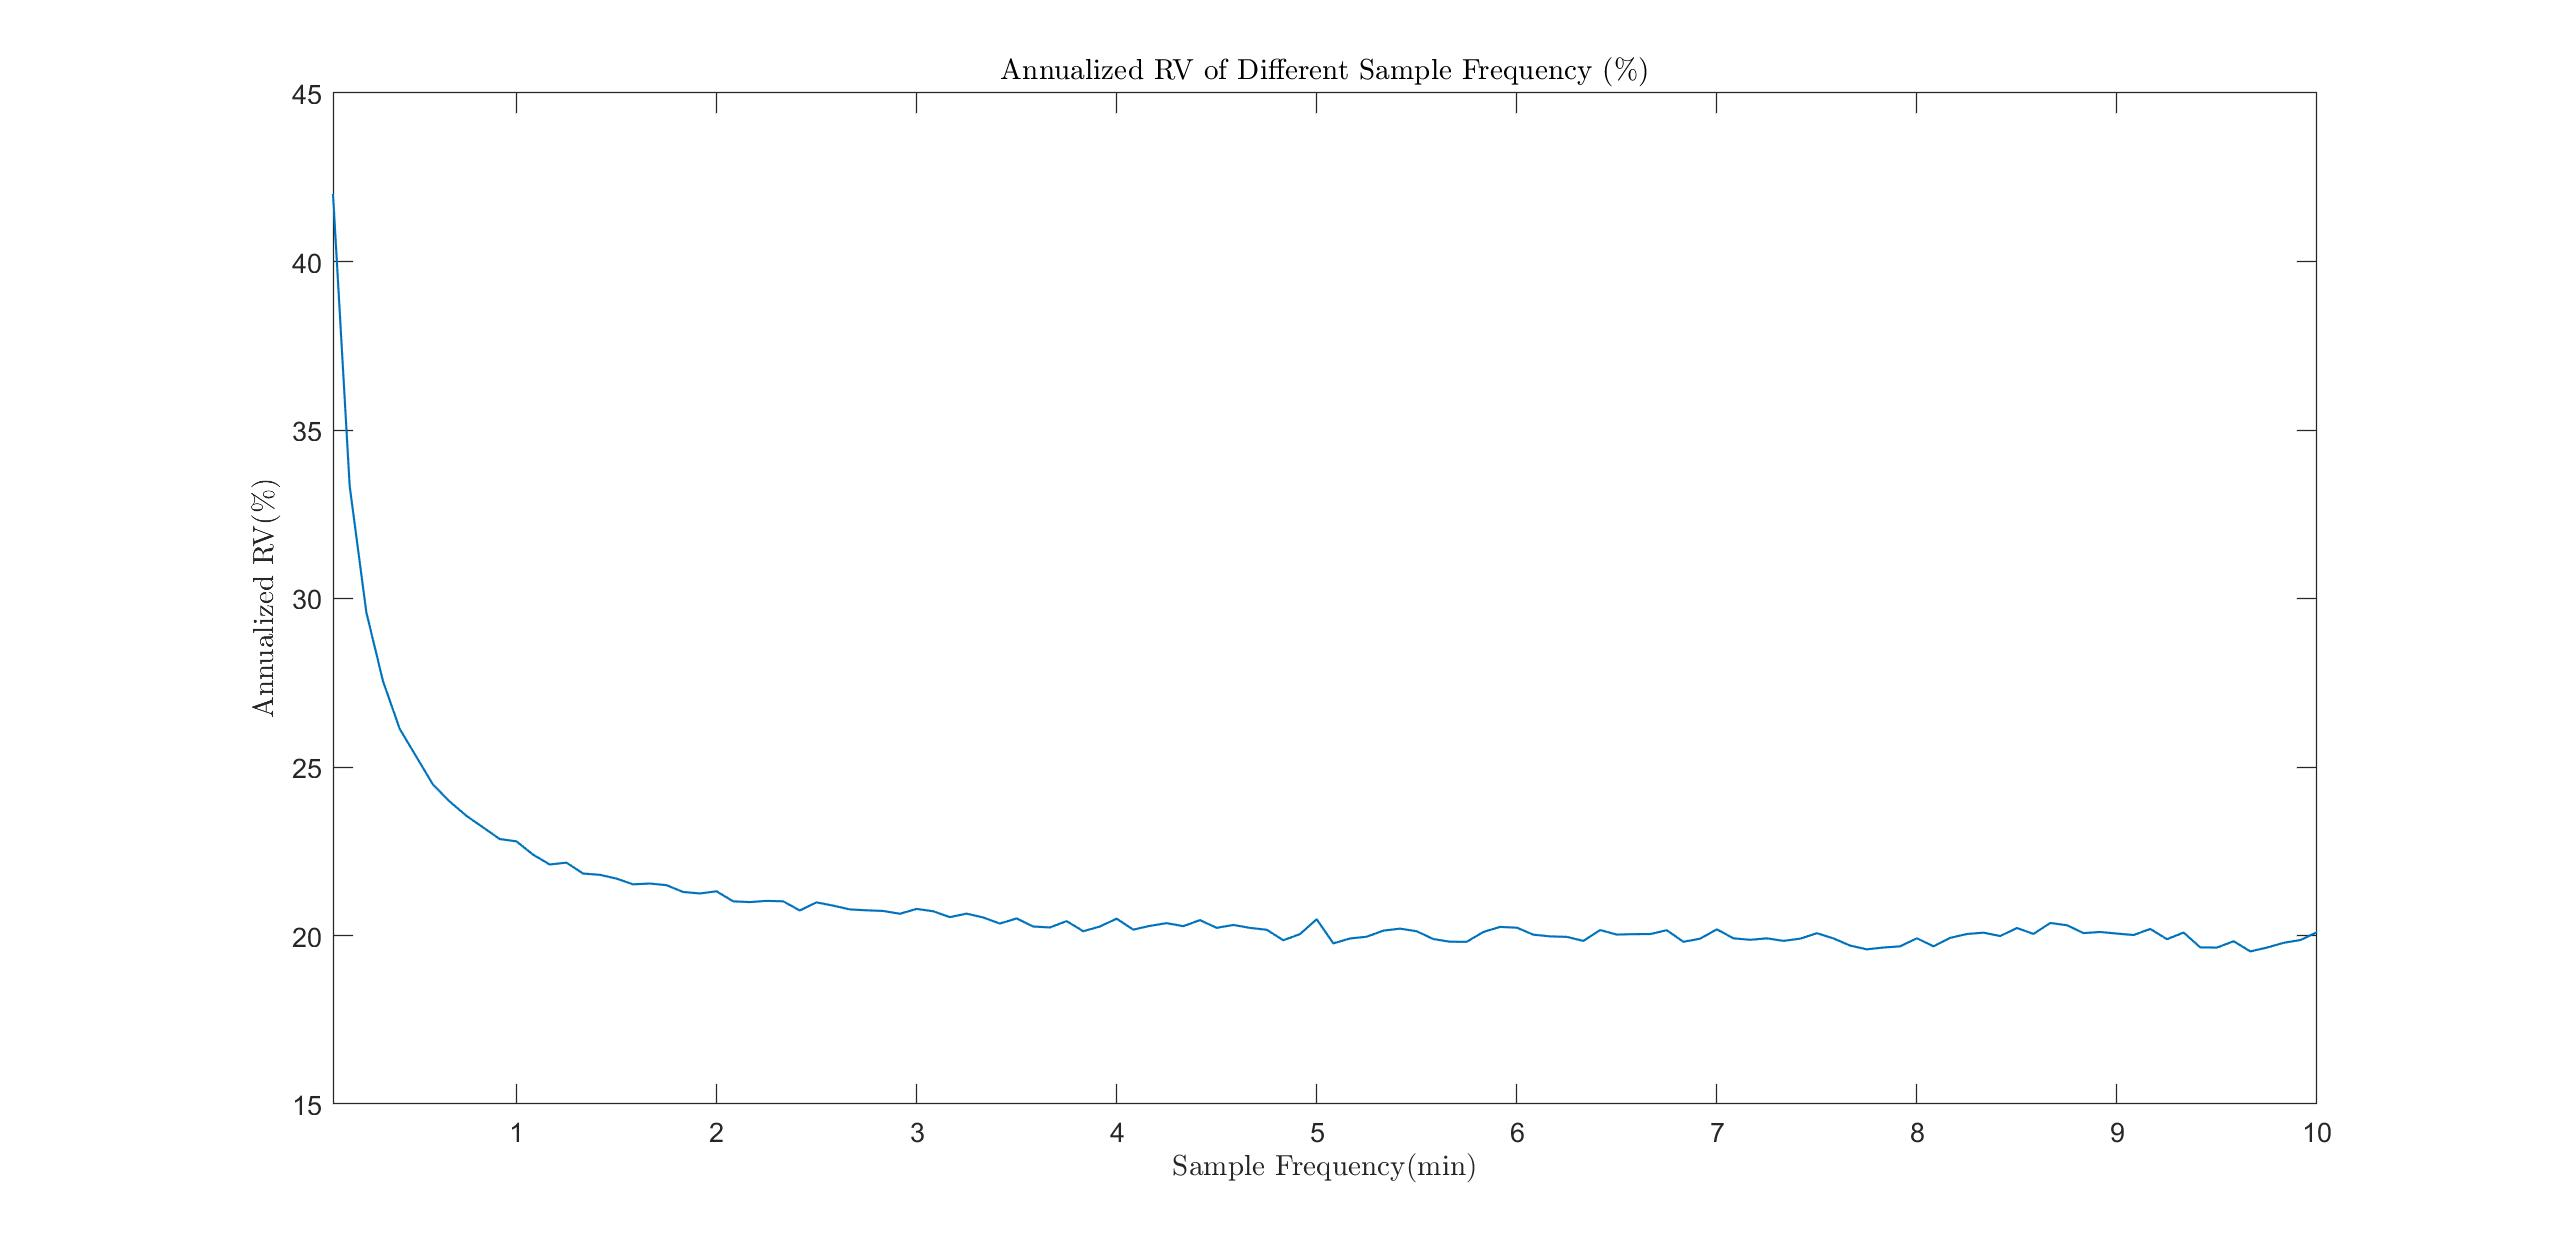
\includegraphics[width=12cm]{figures/ex7_B.jpg}
	\caption{Annualized RV with Different Sample Frequency (\%)}
\end{figure}
From the graph we can find, as the frequency decreases ($k_n$ increases), the value the RV decreases, either. When the data frequency decreases to 2min, the value of RV becomes stable.

Since RV includes two components: $\hat{IV}$ and noise, when the data frequency is quite high, say 5-second, the value of RV computed by stock log-returns will be dominated by the noise part. As the frequency decreases, such as 5-minute, the value of RV become stable and the $\hat{IV}$ will dominate RV (the stable value of RV will be a good estimate of IV).

\item 
According to part B's figure, we can find, when the data frequency is very high, the noise part will dominate RV. Motivated by this fact, the RV we calculate from high frequency data will be a good estimate of noise. In this case, $\hat{IV}$ is the ``noise'' of noise.
%----D
\item 
Assume $ E(\chi_i)=0$ and $Cov(\chi_i,\chi_j)=0 ~(\forall i\neq j)$ and $ Cov(X_{i\Delta_n},\chi_i)=0$, we can write the expression of RV calculated by noise log-return data as: 
\vspace{-5mm}
\begin{center}	
	\begin{align*}
	Y_i^n&=X_{i\Delta_n}+\chi_i\\	
	RV&=\sum_{i=1}^{n/k_n}(\Delta Y_{ik_n}^n)^2\\
	&=\sum_{i=1}^{n/k_n}[(X_{i\Delta_n}-X_{(i-1)\Delta_n})+(\chi_{ik_n}-\chi_{(i-1)k_n})]^2\\
	&\approx \sum_{i=1}^{n/k_n}(\Delta_{ik_n}^nX_i)^2+\sum_{i=1}^{n/k_n}(\chi_{ik_n}-\chi_{(i-1)k_n})^2\\
	&\approx \hat{IV}+2\frac{n}{k_n}\hat{\sigma}_{\chi}^2
	\end{align*}
\end{center}  
where $\hat{IV}$ is the estimate of IV using really log-returns and $2\frac{n}{k_n}\hat{\sigma}_{\chi}^2$ is the noise. 

By the definition of \emph{Contribution}($k_n$), we can have:
$$Contribution(k_n)\equiv \frac{2\frac{n}{k_n}\hat{\sigma}_{\chi}^2}{RV}=\frac{Noise}{IV+Noise}$$
%----E
\item
Here is the figure of estimated average $\widehat{Contribution(k_n)}$.

\begin{figure}[H]
	\centering
	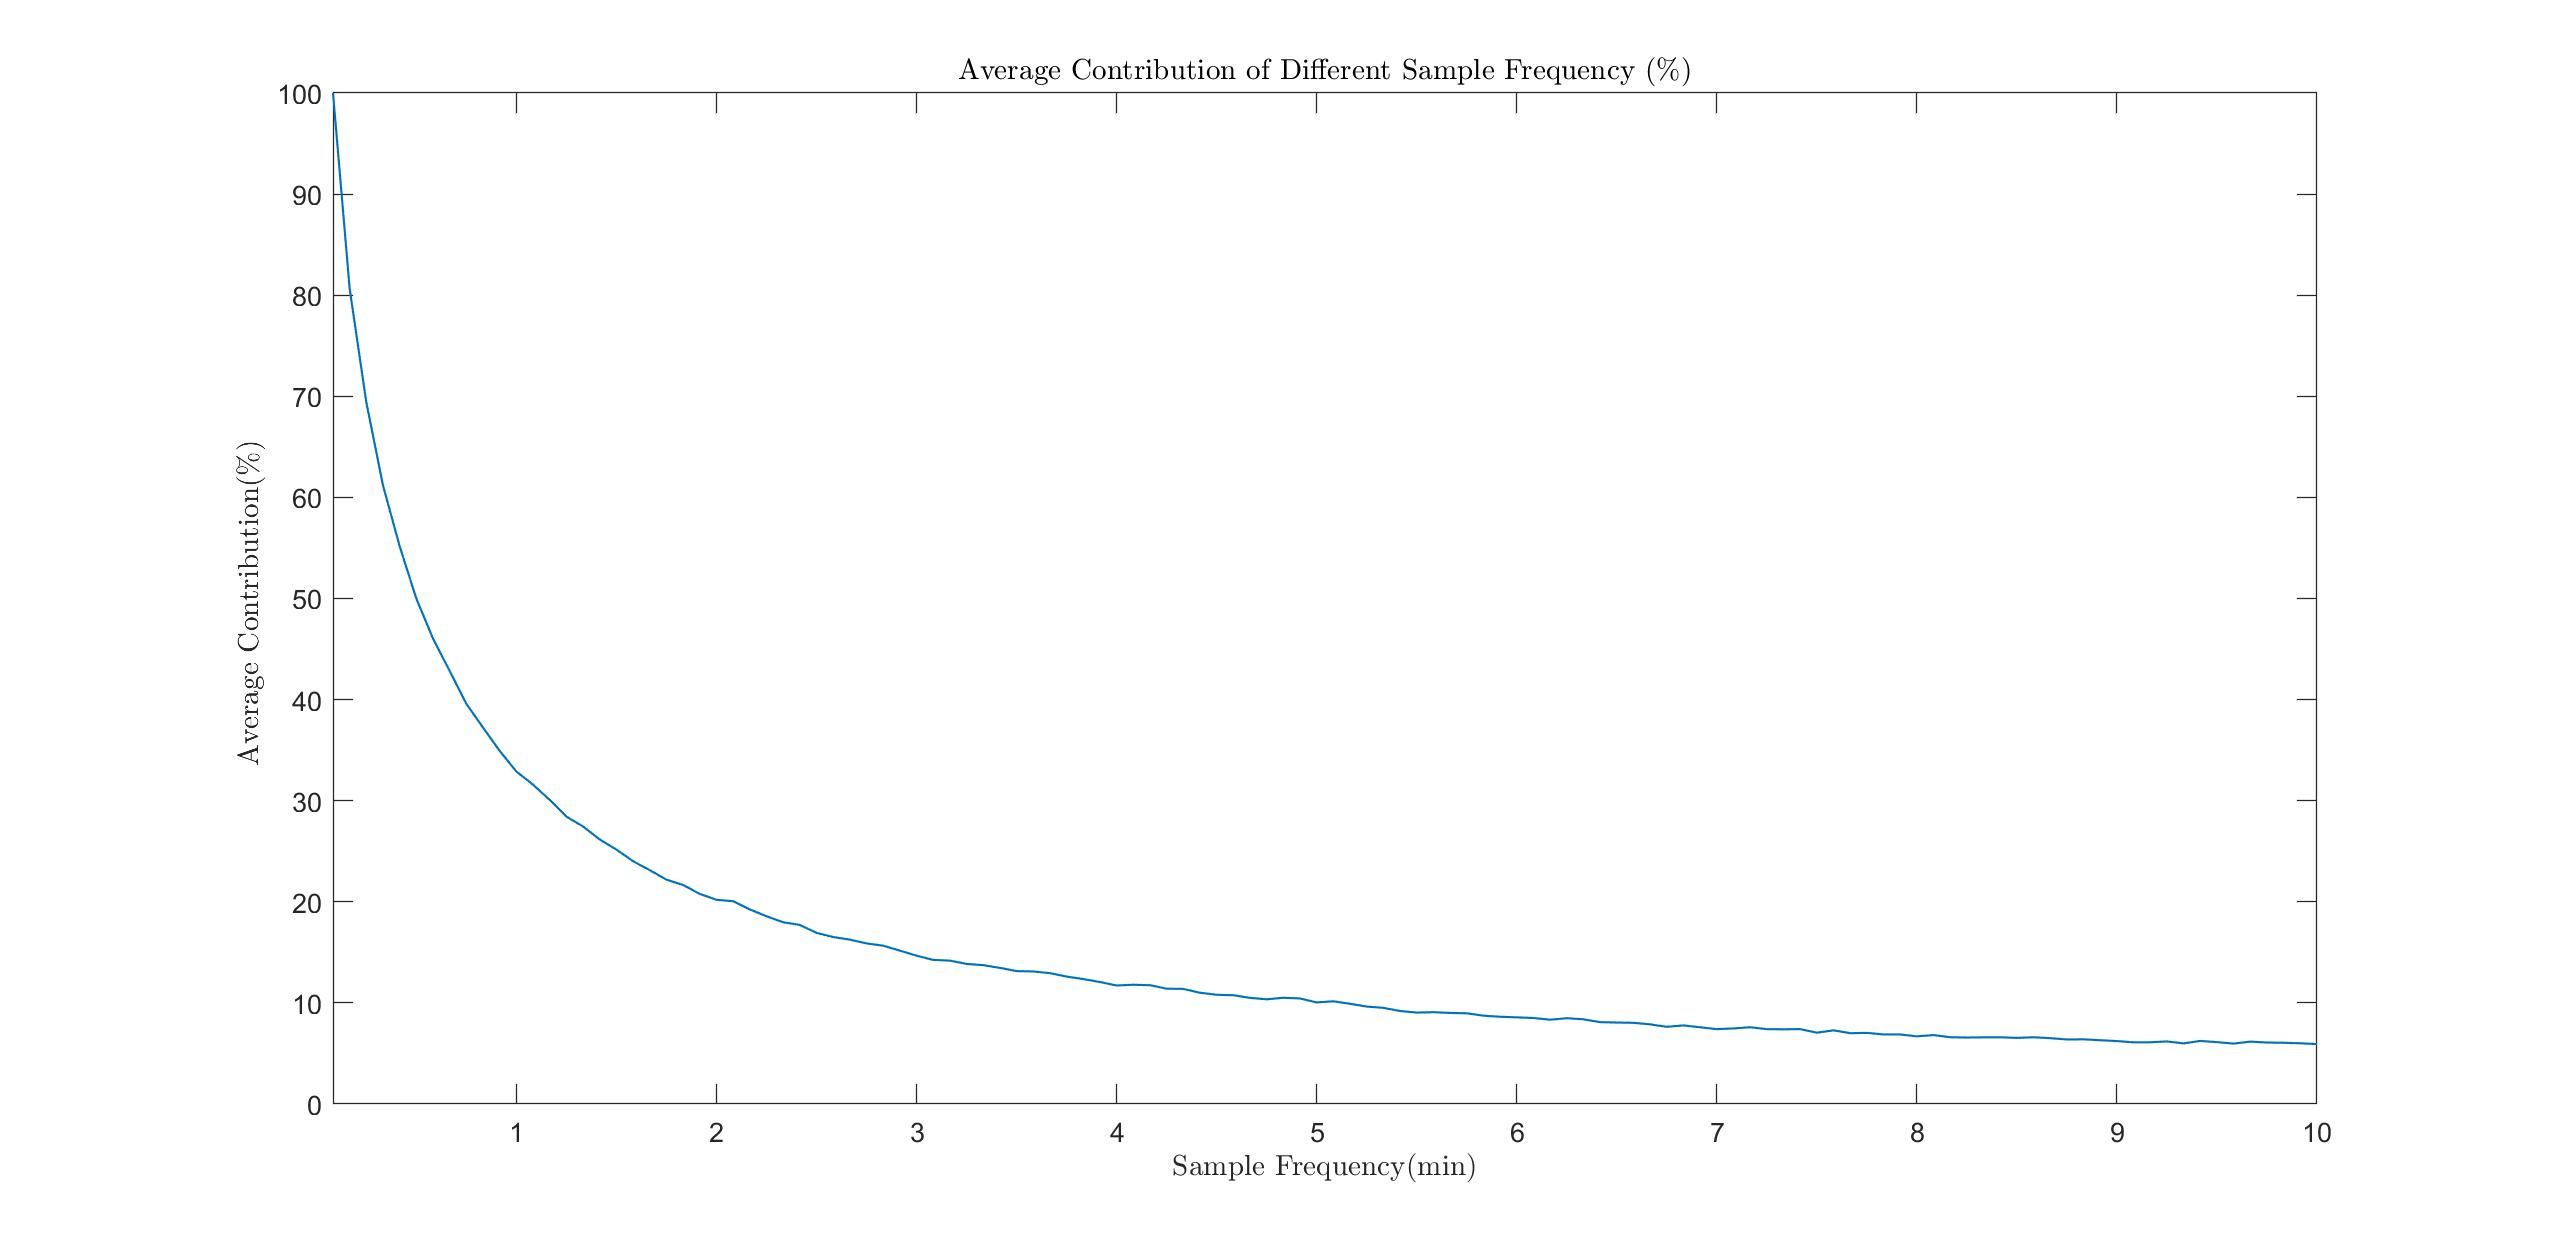
\includegraphics[width=12cm]{figures/ex7_E.jpg}
	\caption{BAC Average Contribution of Different Sample Frequency(\%)}
\end{figure}
From the figure we can see, when the data frequency is really high, the average contribution is close to 100\%, which means the noise will dominate the RV; when the frequency of data decreases to 5-minute (or 8-minute), the contribution will be less than 10\%, which means noise term is unimportant in estimating IV. As the data frequency keeps decreasing, the average contribution decreases further.

%--F
\item
Here is the graph of average RV and coarse sample RV based on 5-minute sample.
\begin{figure}[H]
	\centering
	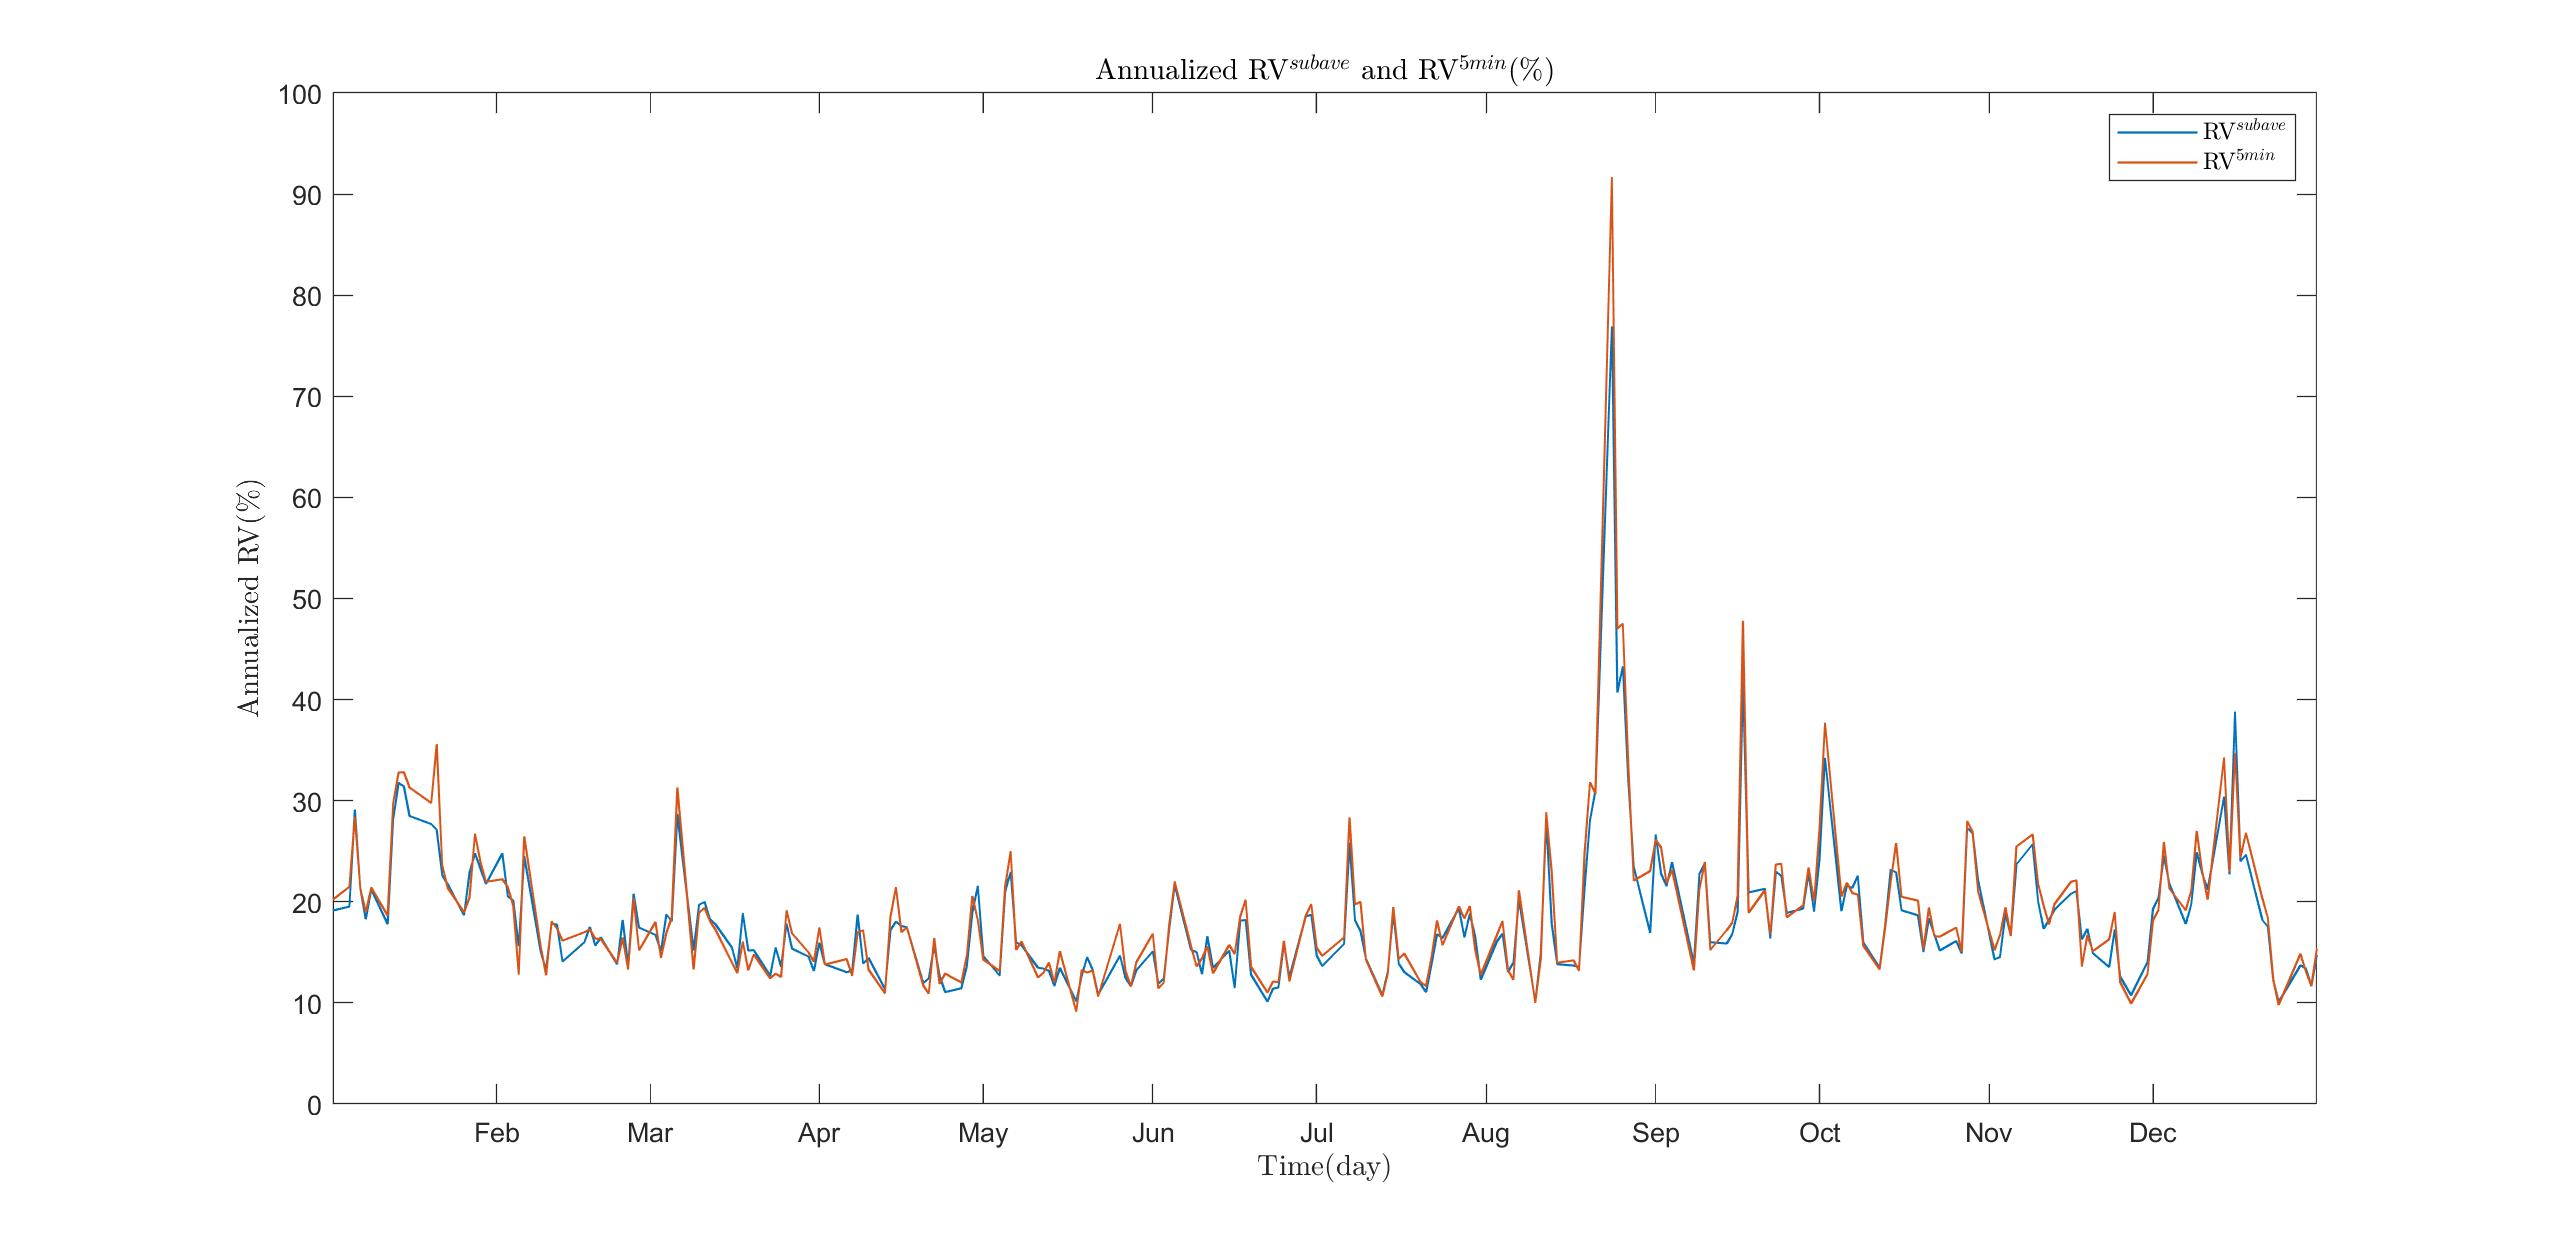
\includegraphics[width=12cm]{figures/ex7_F.jpg}
	\caption{Annualized RV$^{subave}$ and RV$^{5min}$(\%)}
\end{figure}
From the figure we can see, there exists some difference between these two RV even though the difference is very small. Since we use all data to compute TSRV, Tsrv will be a better and more efficient estimator of IV compared to regular RV which only uses coarse sample data.

%--g
\item
Here is the figure of annualized TSRV and RV $^{5min}$.
\begin{figure}[H]
	\centering
	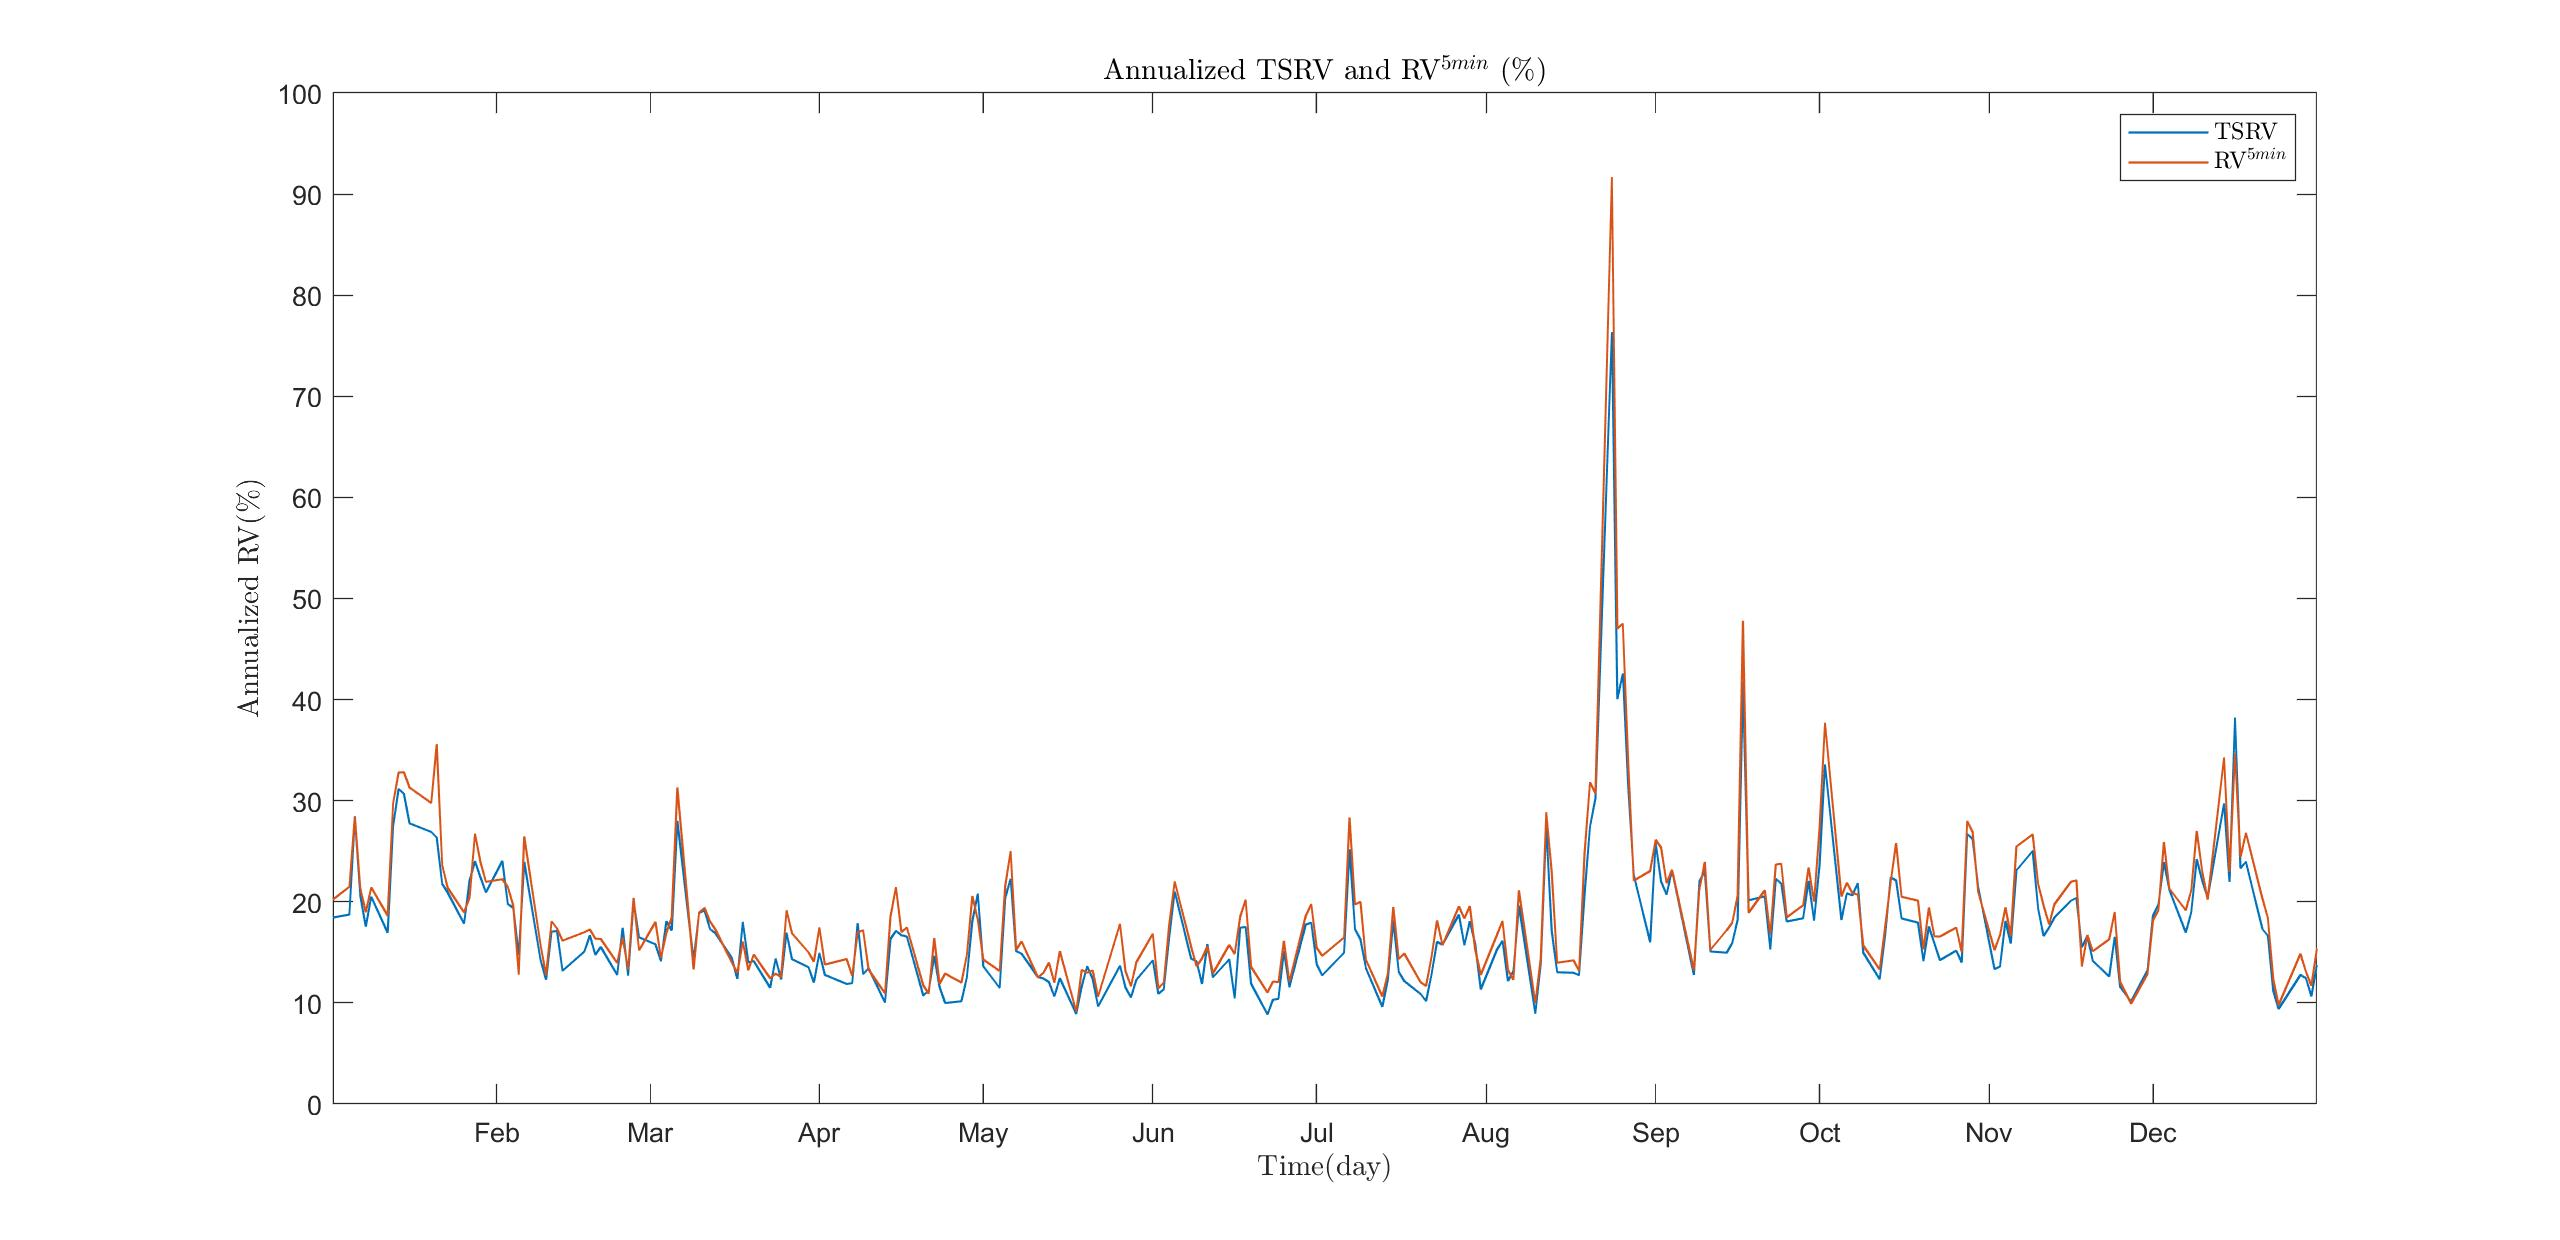
\includegraphics[width=12cm]{figures/ex7_G.jpg}
	\caption{Annualized TSRV and RV$^{5min}$ (\%)}
\end{figure}
According the the figure we can find, the shape of TRSV is very similar to the shape of RV$^{5min}$, which indicates TRSV is a estimator of IV$^{5min}$. However,the value of TRSV is smaller than 5-min RV since we have subtracted noise term from it. After subtracting noises from RV, the value of TSRV will be much closer to IV.

%--h
\item
Here is the figure of Average Annualized TSRV and Volatility with Different Sample Frequency.
\begin{figure}[H]
	\centering
	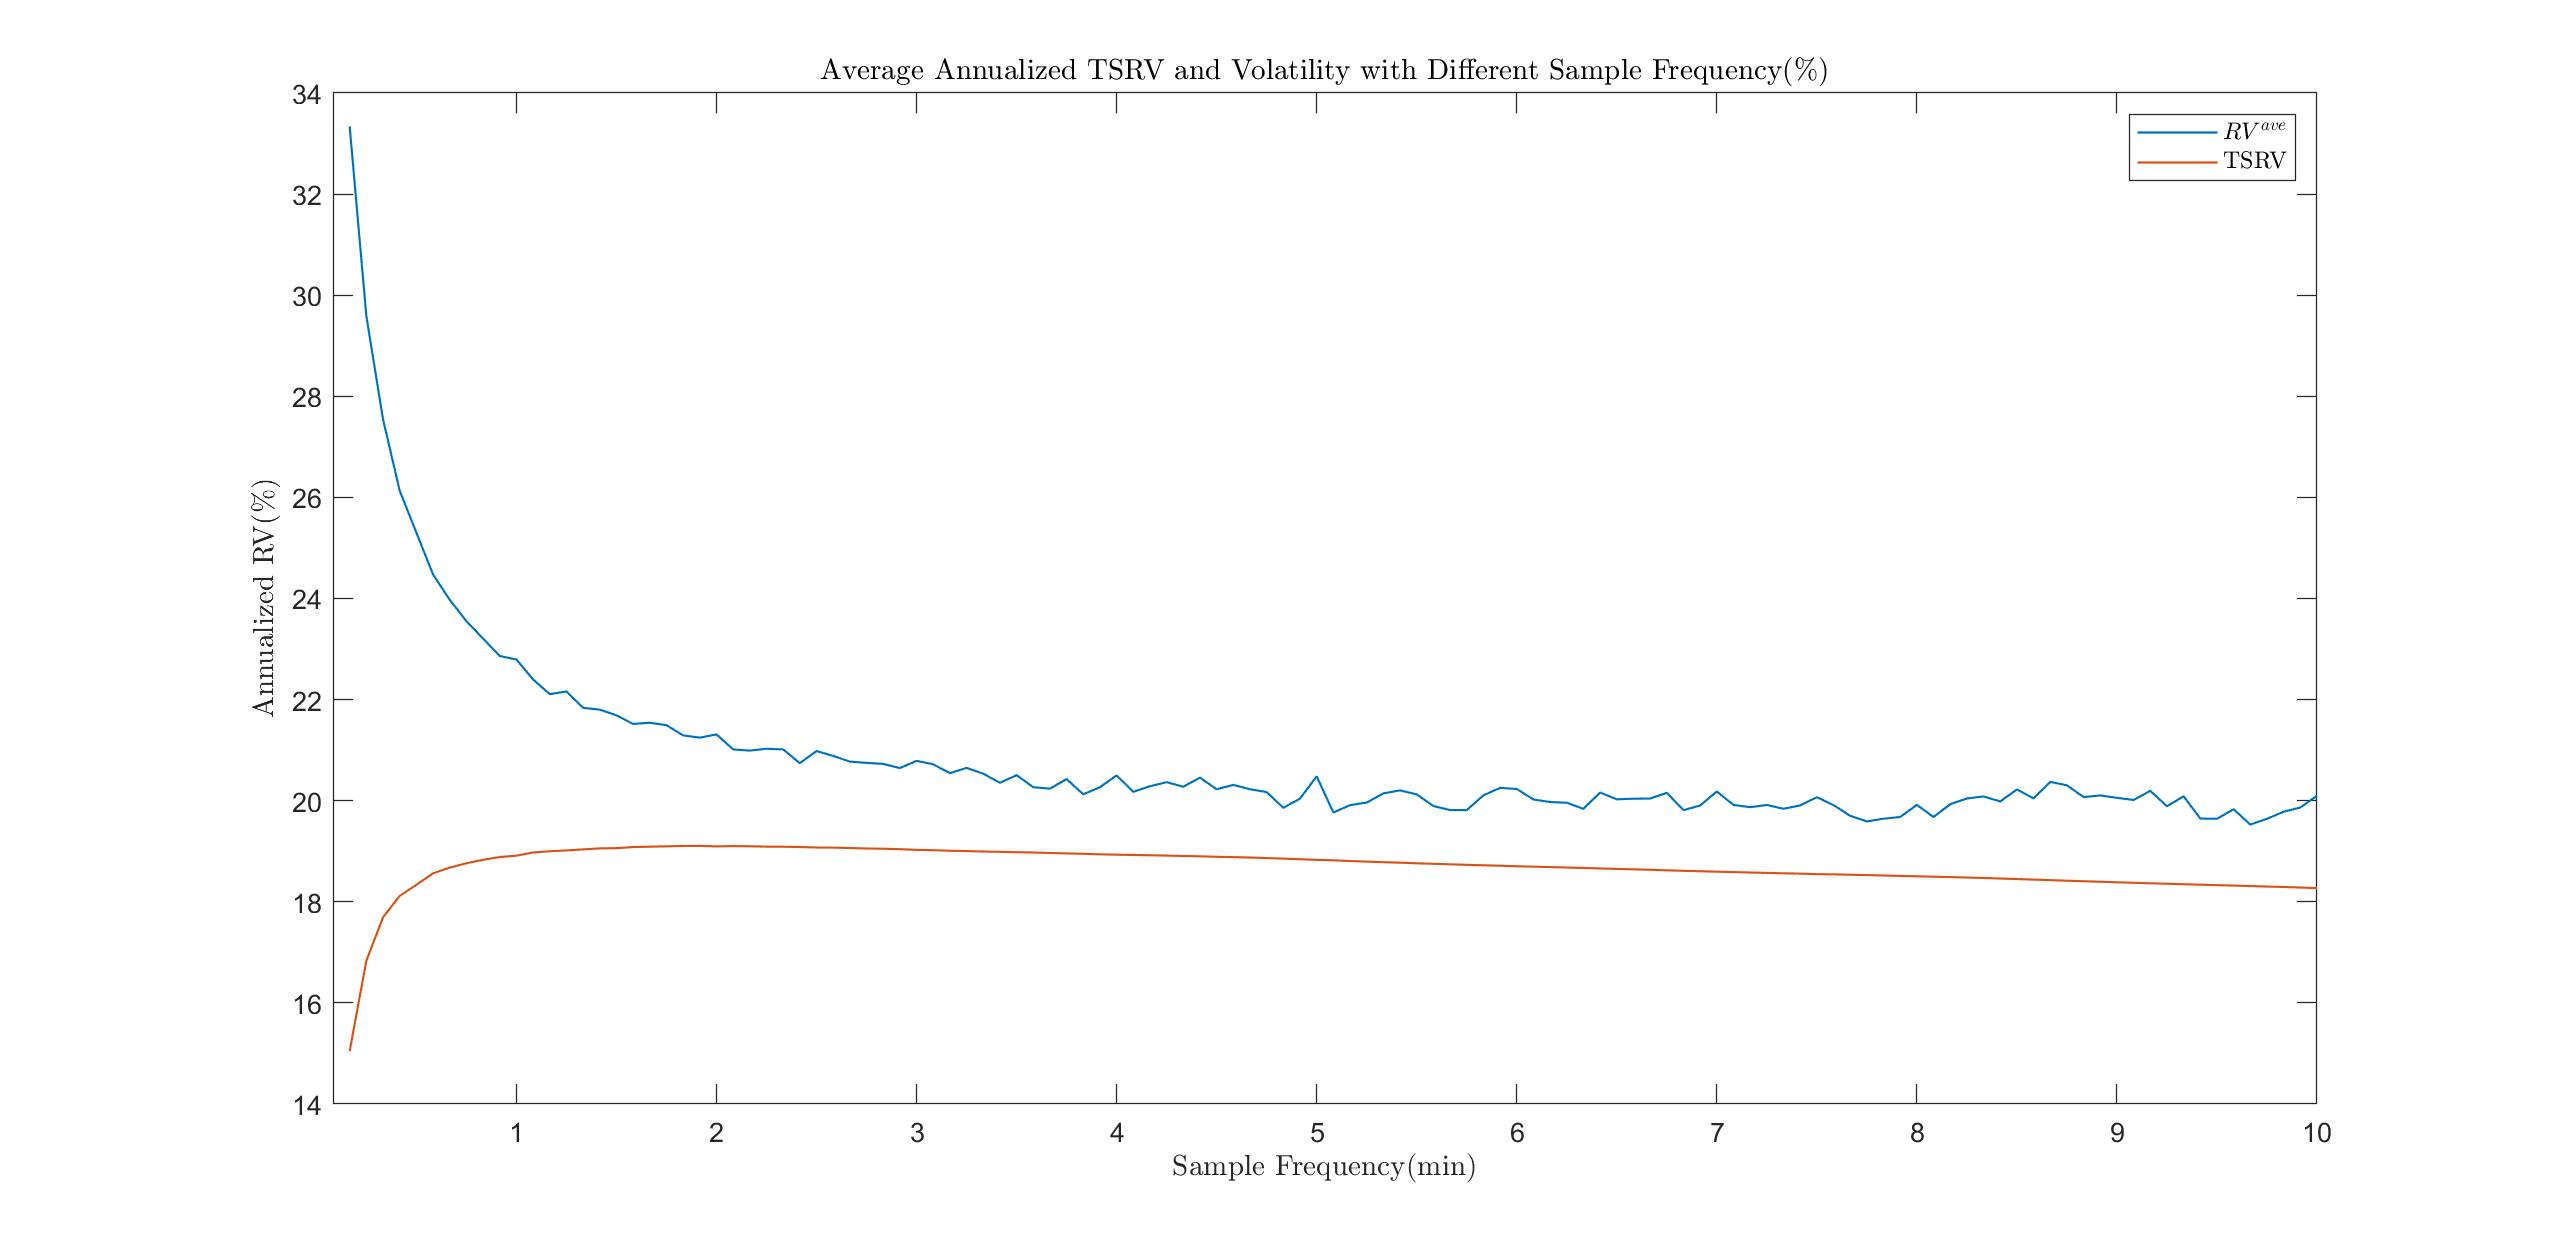
\includegraphics[width=12cm]{figures/ex7_H.jpg}
	\caption{Average Annualized TSRV and Volatility with Different Sample Frequency(\%)}
\end{figure}
For average RV, as the data frequency decreases, its decreases and becomes stable; for TSRV, whose shape is much smoother, as the data frequency decreases, TSRV decreases and becomes stable, too.

 By the definition of TSRV and RV$^ave$, the differences between these two curves are the noise. From graph we can find that, the differences of these two curve becomes smaller as the data frequency goes down, which indicates that the noise proposition in RV$^ave$ becomes smaller. This finding is consistent to the results of contribution figure.\\
\newpage
 



The \textbf{MATLAB} code:

Function of Local Variance
\lstinputlisting{scripts/ex7.m}

\end{enumerate}
 
%---------------------------------------------
\end{document}
